\documentclass{Phyport}

\usepackage{hyperref}
\hypersetup{
    colorlinks=true,
}

\exname{光速测量} %实验名称
\extable{9}
\instructor{乐静飞} %指导教师
\class{github} %班级
\name{MJ} %姓名
\stuid{2025} %学号

\nyear{2025} %年
\nmonth{11} %月
\nday{3} %日
\nweekday{一} %星期几

\begin{document}
\setcounter{page}{0}
\makecover

\section{预习报告（10分）}
\subsection{实验综述（5分）}

本实验使用光调制法，通过测量调制光的相位延迟来确定光的传播时间，从而计算光速。
 
\begin{figure}[htbp!]
    \centering
    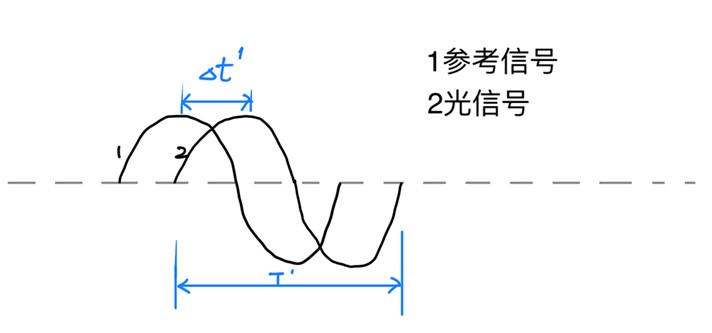
\includegraphics[width=0.3\textwidth]{de.jpg}
\end{figure}

光源发出一个依赖时间变化的周期性光信号，满足：
\[
I = I_0 + \Delta I_0 \cdot \cos{2\pi \nu t}
\]
经一定距离被接收器接收后，接收到的信号相比与原始参考信号有很小的时间延迟，引起相位变化，
通过接收到的信号的相位延迟就能够测量出时间延迟：
\[
\Delta \Phi = 2 \pi \nu \Delta t = \frac{2 \pi \nu \Delta s}{c}
\]
从而光速的计算公式为：
\[
c = \frac{\Delta s}{\Delta \Phi} \cdot 2\pi \nu  
\]

主要测量仪器原理如图：
\begin{figure}[htbp!]
    \centering
    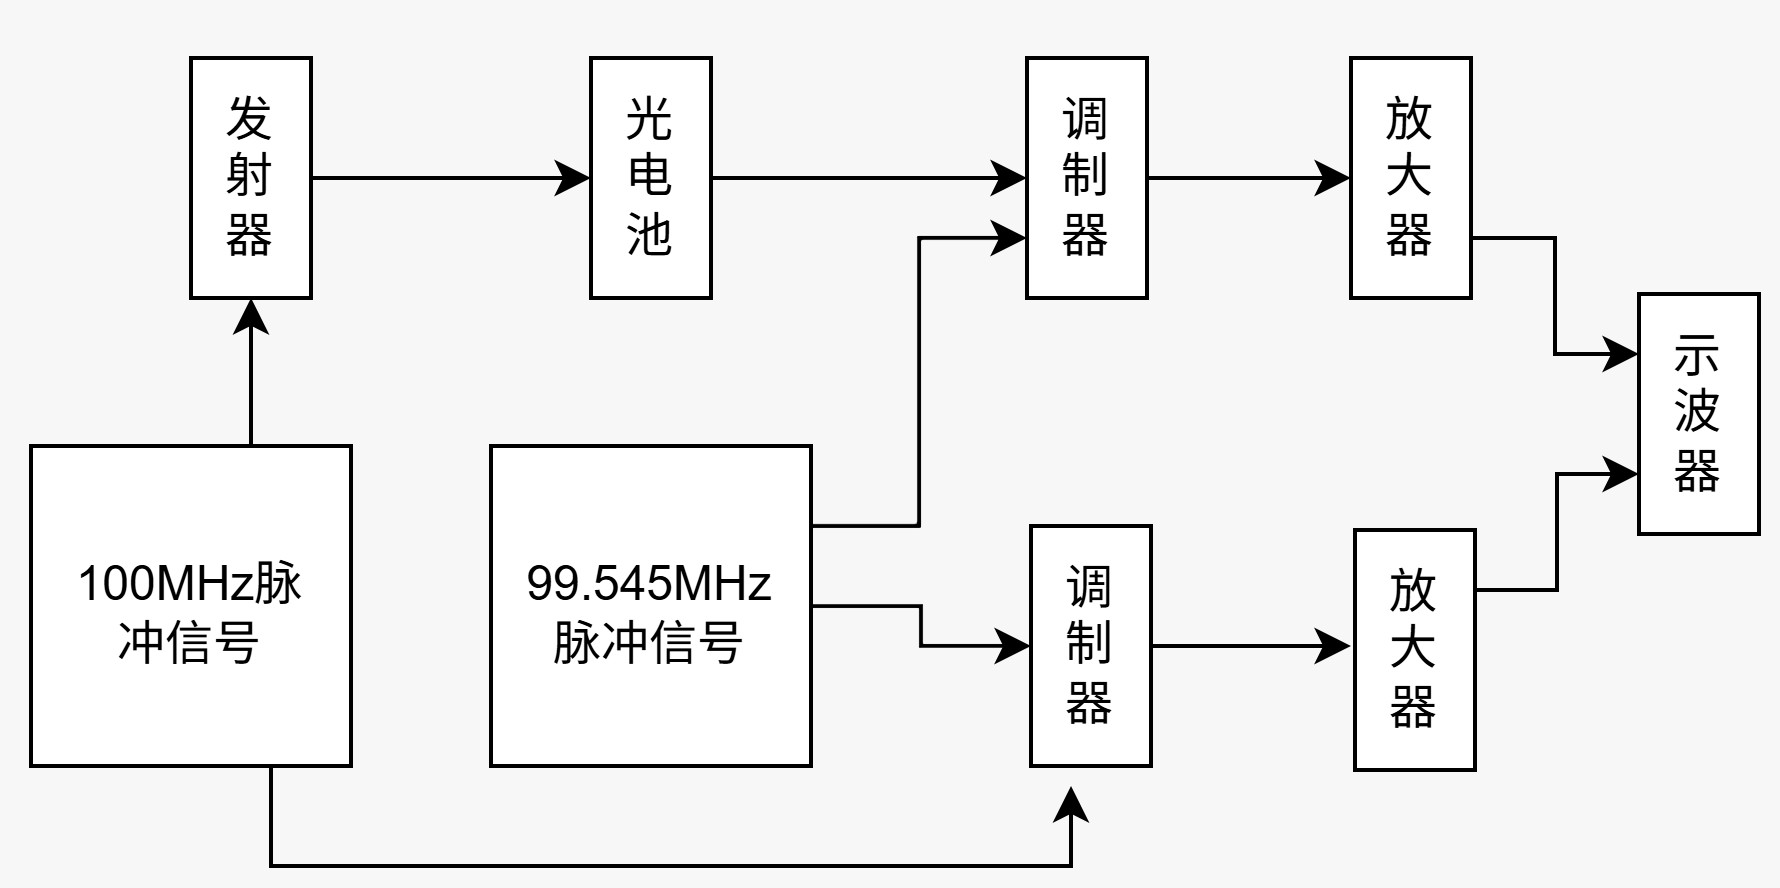
\includegraphics[width=0.5\textwidth]{屏幕截图 2025-11-04 152357.jpg}
\end{figure}

实验时，使用高频调制信号，确保光信号在很短的传播距离下也能获得比较明显的相位变化，
同时要将接收到的信号与另一个信号叠加使示波器显示出该信号。另外为了准确测量相位变化，还有一个参考信号，需调至与接收光信号一致。
然后预先调整光路使得光能被接收器准确接收，输出光源后通过示波器上的输入和输出波形调整光标位置，
在导轨的不同位置多次测量对应的时间间隔 $\Delta t$ ，就能计算光速：
\[
c = 2 \pi \nu \frac{\Delta s}{\Delta \Phi} = \frac{2(S_1 - S_2)}{\Delta t'} \cdot \frac{\nu}{\nu'}
\]

实验过程中，输出调制光后可以在示波器上观察到一个周期性波形，将折光器移动后会发现这个波形有水平移动，
并且时间间隔发生改变；随着折光器位置的改变，相应的时间间隔大致呈线性变化。


\subsection{实验重点（3分）}

本实验的重点在于学会使用示波器测量光波信号时间差，掌握利用光调制法测量光速的基本原理，
了解光信号的调制与解调过程以及光电信号之间的转换。

\subsection{实验难点（2分）}

本实验的难点主要在于对时间延迟的精确测量，由于光速极大，时间延迟非常小，需要分辨率和精度较高的示波器，在移动光标确定波形移动距离时必须准确。
同时要保证光信号发出位置居中，准确返回接收器，基本无偏离，控制噪声干扰，获得可靠的数据。

\section{原始数据（20分）}

\begin{figure}[htbp!]
    \centering
    
\includegraphics[width=0.65\textwidth]{data.jpg}
\end{figure}

\section{结果与分析（60分）}
\subsection{数据处理与结果（30分）}

实验中采用了两种收集数据的方法，并分别用取平均值和作图的方法处理数据，计算光速。

\textbf{1.多次测量求光速}

首先设定
$\nu = 100.0 MHz, \quad \nu' = 454.5 kHz$

\begin{table}[htbp!]
    \centering
\begin{tabular}{|l|l|l|l|l|}
    \hline
    次数 & 初始位置 $S_1 (m)$ & 终止位置 $S_2 (m)$ & $\Delta t' (\times 10^{-9} s)$ & $c (\times 10^{8} m/s)$ \\
    \hline
    1 & 0.0250 & 0.4800 & 649.9 & 3.077 \\
    2 & 0.0250 & 0.5000 & 678.8 & 3.078 \\
    3 & 0.0250 & 0.3500 & 434.4 & 3.291 \\
    4 & 0.0300 & 0.4600 & 605.0 & 3.127 \\
    5 & 0.0300 & 0.4300 & 551.1 & 3.193 \\
    6 & 0.0400 & 0.4500 & 587.0 & 3.073 \\
    \hline
\end{tabular}
\end{table}

求出六次测量后光速的平均值为
\[
\bar{c} = \frac{1}{6} \sum_{i=1}^{6} c_i = 3.140 \times 10^8 m/s
\]

计算 $A$ 类不确定度为
\[
u_A(c) = \sqrt{\frac{1}{n(n-1)} \sum_{i=1}^{n} (c_i - \bar{c})^2} = 3.6 \times 10^6 m/s
\]

因此最后光速测量的结果是
\[
c = \bar{c} \pm u_A(c) = (3.140 \pm 0.036) \times 10^8 m/s  
\]


\textbf{2.等间隔测量}

首先设定
$\nu = 100.0 MHz, \quad \nu' = 454.4 kHz$

\begin{table}[htbp!]
    \centering
\begin{tabular}{|l|l|l|l|l|}
    \hline
    次数 & 初始位置 $S_1 (m)$ & 终止位置 $S_2 (m)$ & $\Delta t' (\times 10^{-9} s)$ \\
    \hline
    1 & 0.0100 & 0.0900 & 117.6 \\
    2 & 0.0100 & 0.1700 & 216.3 \\
    3 & 0.0100 & 0.2500 & 328.5 \\
    4 & 0.0100 & 0.3300 & 449.7 \\
    5 & 0.0100 & 0.4100 & 561.9 \\
    6 & 0.0100 & 0.4900 & 692.1 \\
    \hline
\end{tabular}
\end{table}


以终止位置为纵坐标，时间间隔为横坐标，通过MATLAB对六组数据进行线性拟合，根据作图的斜率计算出光速为
\[
c_k = 3.053 \times 10^8 m/s
\]

对比光速的标准值 $c_0 = 2.997 \times 10^8 m/s$ 计算相对误差为
\[
E = \frac{|c_k - c_0|}{c_0} \times 100\% = 1.87 \%
\]

$A$ 类不确定度为
\[
u_A(c) = 5.9 \times 10^6 m/s
\]

\begin{figure}[htbp!]
    \centering
    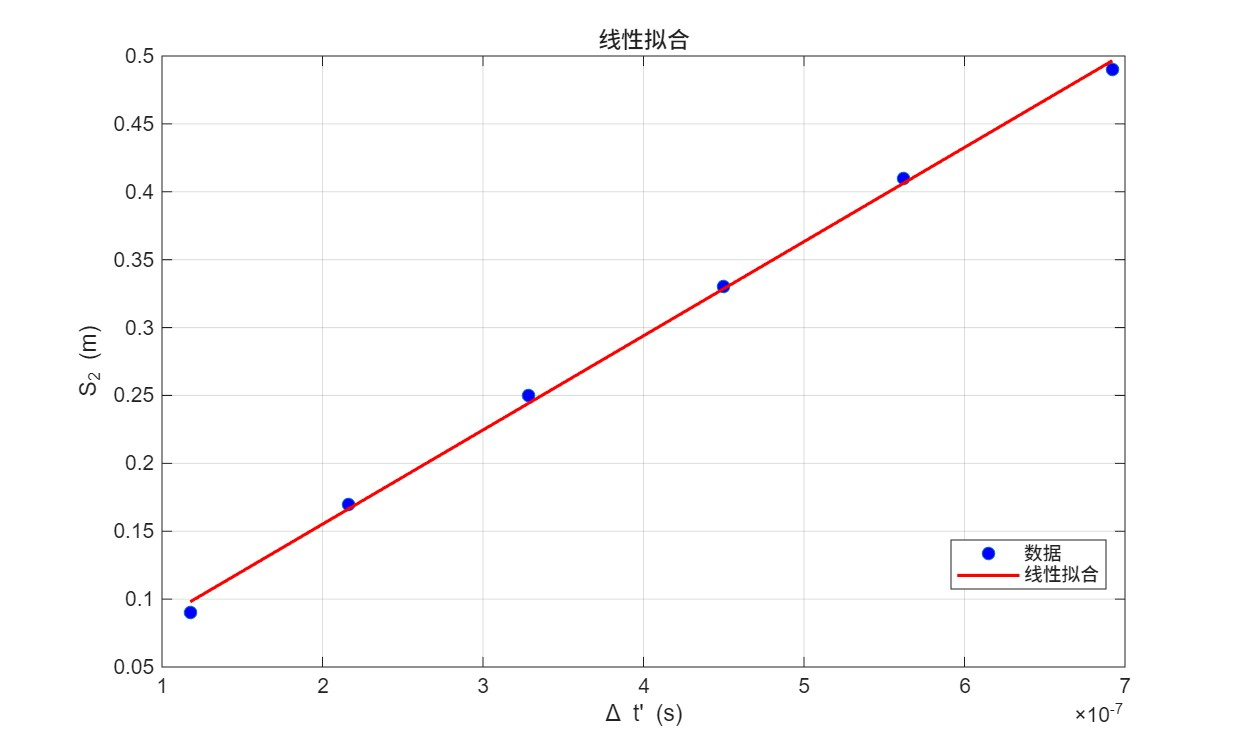
\includegraphics[width = 0.6\textwidth]{fit_c.jpg}
\end{figure}

因此最后光速测量的结果是
\[
c = c_k \pm u_A(c) = (3.053 \pm 0.059) \times 10^8 m/s  
\]

\subsection{误差分析（20分）}

两种数据收集和处理方法测出的光速分别为 $c = (3.140 \pm 0.036) \times 10^8 m/s $ 和 $c = (3.053 \pm 0.059) \times 10^8 m/s$ ，
从结果来看等间隔测量并且进行线性拟合的方法更接近真实的光速，相对误差为 $1.87\%$ ，而多次测量取平均值的
方法相对误差更大一些，这说明使用最小二乘法进行线性拟合的处理数据方法更为可靠和准确。

而两种方法的 $A$ 类不确定都比较大，说明实验过程不够稳定，存在相对强的噪声干扰，随机误差较大。

经过分析，主要误差来源可能有：
\begin{itemize}
    \item 存在系统性偏差，第一组数据求出的光速均明显高于光速的实际值，可能是折光镜没有调整好，光路不完全水平，传播距离有明显误差；
    \item 各组光速测量波动较大，可能是折光器位置的标尺读数有误差，以及测量时间间隔时示波器上两条纵线位置有微小偏差，需要说明的是第一组实验我测了两遍，因为第一遍测量误差过大，发现应当就是由于折光器没有调整好；
    \item 测量系统，包括示波器、脉冲信号等都可能不完全稳定，导致随机误差。
\end{itemize}


\subsection{实验探讨（10分）}

本实验利用光调制法测量光速，实验中以高频信号调制光源，通过示波器显示并测量调制信号在不同光程下的时间差，
从而计算光在空气中的传播速度。实验进行了多次随机测量和等间隔测量两种方法：前者通过多次独立测量取平均值求得光速，后者通过改变光程并作线性拟合求斜率得到光速。
实验中随着光路长度增加，示波器上信号的相位移动逐渐增大，前后波形相对位移明显。最终两次测得光速的相对误差在 $5\%$ 以内，
表明光调制法能较精确地测定光速。


\section{思考题（10分）}

\subsection{实验中有可能出现波形假移位，如何克服？}

本实验中波形假移位是较为常见的系统误差来源之一，它产生的原因主要在于系统内部光电探测器、调制器或示波器信号通道的延迟不一致，
导致输出电信号的相位出现非真实的偏移，从而影响时间差或相位差的测量精度。假移位还可能来自光电信号幅度过低、信噪比较差、或信号波形失真等因素。

为克服这一问题，应首先进行示波器校准，保持信号路径对称与一致，确保电缆长度、接触电阻与通道延迟相同；其次，应提高信噪比，
通过调整光强、加装滤波器等手段来减少噪声干扰；再次，应校正系统延迟，可通过零光程差下的相位对比进行基线修正；
当然以上方法主要是在调整测量系统，实验中应使用测量相位差的办法相减抵消假位移，还可以多次独立重复测量，以减弱随机误差影响。
以上措施应当能够降低假移位带来的系统误差，提高光速测量的准确度。

\subsection{分析影响实验精度的主要因素}

本实验中，影响实验精度的因素主要包括仪器性能、环境条件及实验操作等多个方面。

首先，时间测量精度是决定结果可靠性的关键因素。由于实验中的时间差在纳秒量级，若示波器的时间分辨率有限或触发不稳定，
就会引入较大的随机误差；而且这个时间间隔的两条纵线是手动确定的，微小位移就会导致时间产生变化，容易产生比较大的误差；
同时还必须校准光信号的发出和接收通道，保证光点在发射器和接收器的中央，否则误差会非常大。

其次，光程的测量，即折光镜的位置测量用的标尺是毫米级的，精度较低，读数时也可能造成误差。

再次，光电信号质量与信噪比直接影响波形判断的准确性。若光源强度不稳、探测器灵敏度不足或线路噪声较大，
信号波形易出现畸变或漂移，导致假移位现象，进而降低精度；而如果调制信号的频率不稳定，也会引入系统误差。

再次，系统延迟与仪器非理想特性，如电缆长度差异、放大器相移等都会产生系统误差，
使测量相位差与真实值不符。

此外，环境因素如空气折射率随温度、湿度变化，也可能会对光速值产生微小影响，不过在本实验中应该还没有达到要考虑环境干扰的精度。

总而言之，提高实验精度需在仪器校准、信号调制优化及测量方式等方面综合改进，以减小系统误差和随机波动。

\subsection{描述光速测量的其他方法}

早期的光速测量方法主要是天文学方法，利用光在遥远天体间的传播所需时间间隔
粗测光速。奥勒·罗默首次测定光速就是通过研究木卫一的视运动，观测木星卫星被木星遮挡的时间变化来推算光速：由于光程变化
而产生时间延迟，当光程变化为 $\Delta L$ （根据地球与木星的相对运动这个距离一般为地球轨道的直径），实际观测到的时间比预期延迟 $\Delta t$ 时，光速为
\[
c = \frac{\Delta L}{\Delta t}
\]

更精确的测法主要是大地测量法，通过高速机械装置较为准确地测量光传播时间。
迈克尔逊的旋转棱镜法就是使用高速旋转的多面棱镜，确保光往返一段距离总长 $L$ 时所经过的时间 $t$ 恰好等于旋转棱镜转过 $\frac{1}{N}$
个面所需的时间，那么光速为
\[
c =\frac{L}{t}
\]

现代光速测量主要使用精度极高的电子与光学方法，一般依据电磁学理论和相对论原理，借助波的一些性质。
最常见的是使用高度稳定的激光器，精确发射频率稳定为 $f$ 的激光并用干涉仪或共振腔法等手段测定波长 $\lambda$ ，
计算出光速为
\[
c = f \cdot \lambda
\]

\begin{thebibliography}{9}
    \bibitem{ref1}
    陈水桥,刘万生,陈洪山. 调制法测量光速[J]. 物理实验,2004,24(10):6-8. DOI:10.3969/j.issn.1005-4642.2004.10.002.

    \bibitem{ref2}
    陈宝骥,韦先涛,王中平. 基于光学多普勒效应的光速测量与监听实验[J]. 物理实验,2023,43(5):37-42. DOI:10.19655/j.cnki.1005-4642.2023.05.006. 

    \bibitem{ref3}
    刘义保,邓玲娜,黎定国,等. 多道时间谱仪测量光速[J]. 物理实验,2005,25(6):3-5. DOI:10.3969/j.issn.1005-4642.2005.06.001. 

    \bibitem{ref4}
    王绶琯. 从罗默的光速测量说起[J]. 物理通报,2006(8):1-2. DOI:10.3969/j.issn.0509-4038.2006.08.001. 

    \bibitem{ref5}
    陈水桥,陈洪山. 利用铜激光与光纤技术测量光速[J]. 物理实验,2003,23(4):10-12. DOI:10.3969/j.issn.1005-4642.2003.04.003. 
\end{thebibliography}

\input{注意事项}
\end{document}
